
%-----------------------------------------------------------------------------
% Chapter: Development
%-----------------------------------------------------------------------------

\chapter{Development}
\label{chap:DEV}

\section{Methodology}
The most important point in the development process of the \emph{Course2018}
LMS is the idea of \emph{continuous integration} (CI), meaning that every new
develop feature is tested and integrated to the existing server seamlessly.

\medskip
This is achieved by using a development tool called \emph{GitLab CI}
\cite{gitlabCI}, a sub-system that came with the source management tool,
\emph{GitLab}~\cite{gitlab}, which is also used for the development of this
project. 

\medskip

This tool chain offers abilities to a developer so that every time
the developer finishes programming of a feature and pushes the code to the
\emph{GitLab} project repository, the \emph{GitLab} server automatically
invokes some
routines to test the new code with a test scheme also defined by the developer
prior to the time when the code was pushed; if all tests are passed, 
the \emph{GitLab} server then deploys the new version of the project by simply
building a new container that has the latest code in it, and has the old
container replaced with the new one. 

\section{Deployment}
In the development process of this project, the deployment stage is defined
before the actual programming even start. This approach makes sure that all
modules of the project can be test in the
deployment environment (i.e., the container in which the \emph{Course2018}
will be eventually running) as soon as the implementation if finished.

\subsection{Environment}
The \emph{Course2018} LMS is containerized in an environment
(the production container) based on
\emph{Debian 8}~\cite{debian}, with \emph{Python 3} and all necessary packages
(including \emph{Django 2.0}) installed.

\subsection{HTTP server}
An \emph{HTTP server} is included in the production container to host the
\emph{Course2018} LMS.
The \emph{HTTP server} in use in the production container is the
\emph{Apache HTTP server} (version 2.4)~\cite{apache}, with the
\texttt{mod\_wsgi}~\cite{wsgi} package installed to accommodate
\emph{Python} web applications in \emph{WSGI}
(Web Server Gateway Interface~\cite{wsgi}) specification, such as a
\emph{Django} project.

\section{System development}

\subsection{MVT}
\label{sec:MVT}
The \emph{Django} framework enforces developers to apply an architectural
pattern called the \emph{MVT} (Model-View-Template) pattern to their projects.
In such projects,
all data models are defined as \texttt{Model} classes, which
then are used to create schemas for corresponding database tables;
the data in the data models will then be retrieved and organized in 
methods of different \texttt{View} classes, each of these \texttt{View} classes
is connected to a \emph{URL};
webpages will finally be generated by those \texttt{View} classes
using different \emph{HTML} \texttt{Templates} with the organized data.

\subsection{APIs}
In the \emph{Course2018} LMS, some views are not paired with templates, and
they do not return webpages to the users, instead, they return some
\emph{JSON}-formatted data.
These views are the application programming interfaces (APIs) of the system,
and they are used for updating information in
a loaded page dynamically with \emph{AJAX}~\cite{AJAX}. 


%-----------------------------------------------------------------------------
% Section: User authentication
%-----------------------------------------------------------------------------

\subsection{User authentication}
As discussed in Section~\ref{sec:USRAUTH}, user authentication is handled by the
\emph{Django User Model} provided by the \emph{Django} \texttt{auth} library,
not only does this approach simplifies the implementation of the module,
security is also improved in comparison with implementing the authentication
module solely by the developer.

\subsubsection{Data model}
Data model of the user authentication module is shown in
Figure~\ref{fig:AUTH_ER}, Table~\ref{tab:USR_ATTR} and
Table~\ref{tab:PROFILE_ATTR}.

\bigskip

\begin{figure}[ht]
    \centering
    \caption{Data model of the user authentication module}
    \usetikzlibrary{er}
    \label{fig:AUTH_ER}

    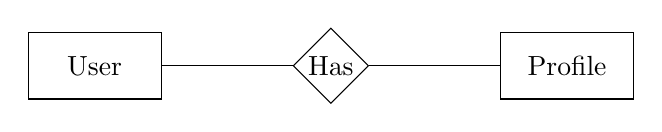
\begin{tikzpicture}[node distance = 3cm]
        \node[entity] (user) {User};
        \node[relationship] (has) [right of=user] {Has} edge (user);
        \node[entity] (profile) [right of=has] {Profile} edge (has);
    \end{tikzpicture}
\end{figure}


\begin{table}[ht]
    \centering
    \caption{Attributes of \texttt{User} model}
    \label{tab:USR_ATTR}
    \renewcommand{\arraystretch}{1.5}
    \begin{tabular}[ht]{r|l}
        \hline
        Attribute & Note \\
        \hline
        \hline
        \texttt{id} & primary key \\
        \hline
        \texttt{username} &  required, max length: 150 \\
        \hline
        \texttt{first\_name} &  optional, max length: 30 \\
        \hline
        \texttt{last\_name} &  optional, max length: 150 \\
        \hline
        \texttt{email} & optional\\
        \hline
        \texttt{password} & A hash of the user's password \\
        \hline
        \texttt{is\_active} & \texttt{boolean field}, indicating whether or not the user
            is active \\
        \hline
        \texttt{last\_lgoin} & \texttt{datetime field}, last login time \\
        \hline
        \texttt{data\_joined} & \texttt{datetime field}, time when the account is created \\
        \hline
    \end{tabular}
    \renewcommand{\arraystretch}{1}
\end{table}

\begin{table}[ht]
    \centering
    \caption{Attributes of \texttt{Profile} model}
    \label{tab:PROFILE_ATTR}
    \renewcommand{\arraystretch}{1.5}
    \begin{tabular}[ht]{r|l}
        \hline
        Attribute & Note \\
        \hline
        \hline
        \texttt{user\_id} & foreign key to a \texttt{User} model instance \\
        \hline
        \texttt{role} & \texttt{integer field}, choice from 0 and 1, indicating the
            user's role \\
           & is \emph{Student} or \emph{Professor} respectively \\
        \hline
    \end{tabular}
    \renewcommand{\arraystretch}{1}
\end{table}


\subsubsection{Views}

\begin{itemize}
    \item Login: \\
        A \texttt{UserLogin} view is defined to provide routines to handle user
        authentications, by invoking the built-in \emph{Django} library
        function~\texttt{authenticate()}
        to compare the credentials provided
        by the user against the user account database.

    \item Permission control: \\
        An abstract view class called \texttt{AbstractLoginRequiredView} is
        defined for general permission control. This class contains a function
        to check whether or not a user is authenticated, if the user is
        authenticated, the function then checks the role of the user and
        invokes \texttt{student\_view()} or \texttt{professor\_view()} to
        provide different content according to the user's role.

        All the views of the modules that require permission control are
        inherited from the \texttt{AbstractLoginRequiredView} class, and have
        the class function \\ \texttt{student\_view()} and
        \texttt{professor\_vew()} overridden to provide module-specific
        content for students and instructors respectively.

        In addition to that, there is also another abstract view class, \\
        \texttt{AbstractAPI}, this class provides permission
        control for all the APIs in the same manner as discussed above.
\end{itemize}

\subsubsection{Templates}

\begin{itemize}
    \item Login template: \\
        This template is used by the \texttt{UserLogin} view to provide a very
        simple login interface to the users, it contains a form with two
        fields (username and password) and a \emph{Login} button. User can
        use this interface to log into the \emph{Course2018} LMS.
\end{itemize}


%-----------------------------------------------------------------------------
% Section: Course management
%-----------------------------------------------------------------------------

\subsection{Course management}
To provide source code management for programming assignments,
a great open-source version control tool,
\emph{Git}, is integrated to the \emph{Course2018} LMS,
this was originally developed by \emph{Linus Torvalds}~\cite{git},
creator and principal developer of the \emph{Linux} operating system
kernel~\cite{lTorvalds}.
Moreover, 
an open-source Git-repository manager, \emph{GitLab}~\cite{gitlab}, is also
used in the \emph{Course2018} LMS to enhance the source code management user
experience.

\medskip
Once an instructor enables source code management for an assignment, a remote
\emph{GitLab} repository is also created for the course to which the assignment
belongs. The name of the repository will be saved in the course management
module.

\medskip
Note that course materials feature is planned but not implemented due to the
limit of development time frame (see section {\bf TODO: REF FUTURE WORK}).

\subsubsection{Data model}
Data model of the course management module is shown in
Figure~\ref{fig:COURSE_ER} and Table~\ref{tab:COURSE_ATTR}. \bigskip

\begin{figure}[ht]
    \centering
    \caption{Data model of the course management module}
    \label{fig:COURSE_ER}
    \usetikzlibrary{er}

    \begin{tikzpicture}[scale=0.8, every node/.style={scale=0.8}, node distance = 4cm]
        \node[entity] (course) {Course};

        \node[relationship] (stu_reg) [below of=course] {Student} edge[total] (course);
        \node[entity] (stu) [left of = stu_reg] {User (Role: student)} edge[total] (stu_reg);

        \node[relationship] (instructor) [above of = course] {Instructor} edge (course);
        \node[entity] (prof) [left of = instructor] {User (Role: professor)} edge (instructor);

        \node[relationship] (ta_reg) [right of = course] {TA} edge[total] (course);
        \node[entity] (ta) [right of = ta_reg] {User} edge[total] (ta_reg);
    \end{tikzpicture}
\end{figure}

\begin{table}[ht]
    \centering
    \caption{Attributes of \texttt{Course} model}
    \label{tab:COURSE_ATTR}
    \renewcommand{\arraystretch}{1.5}
    \begin{tabular}[ht]{r|l}
        \hline
        Attribute & Note \\
        \hline
        \hline
        \texttt{id} & primary key \\
        \hline
        \texttt{department} & required, department code of the course \\ & (e.g., COMP, MATH) \\
        \hline
        \texttt{number} & required, course number \\
        \hline
        \texttt{section} & required, course section (e.g., X1) \\
        \hline
        \texttt{title} & require, course title \\
        \hline
        \texttt{semester} & required, semester of the course (e.g., Winter, Fall) \\
        \hline
        \texttt{start\_time} & required, \texttt{date} field, date the course
            becomes available to \\ & students \\
        \hline
        \texttt{end\_time} & required, \texttt{date} field, date the course ends \\
        \hline
        \texttt{visible\_after\_end} & required, \texttt{boolean} field, indicating
            whether or not to allow\\ & students access the course after it ends \\

        \hline
        \hline

        \texttt{instructor} & foreign key to the instructor \\
        \hline
        \texttt{students} & many to many relationship to the students registered \\ & in the course\\
        \hline
        \texttt{TAs} & many to many relationship to the TAs registered \\ & in the course \\

        \hline
        \hline

        \texttt{repo\_name} & optional, the name of the remote \emph{GitLab}
            repository \\ & in 
            which programming assignment source code files \\ & are stored \\
        \hline
        \hline

        \texttt{constraints} & 
            1. combination of fields
                \texttt{department},
                \texttt{number},
                \texttt{section}, \\ &
                \hspace{1.3em}\texttt{year},
                \texttt{semester} must be unique \\
            & 2. role of the \texttt{instructor} must be \emph{Professor} \\
            & 3. role of the each of the \texttt{students} must be \emph{Student} \\
        \hline
    \end{tabular}
    \renewcommand{\arraystretch}{1}
    
\end{table}

\subsubsection{Views}

\begin{itemize}
    \item Create courses: \\
    \label{item:NEW_COURSE}
        This activity is handled with the \texttt{CreateCourseView} which is
        inherited from the \texttt{AbstractLoginRequiredView} and 
        only accessible by instructors. 
        This view accepts all the \emph{create course} requests, validates the
        data in each of the requests, and if the data has no error,
        create course records with the data in the course database table.
        The permission control of this view
        (and any other views that are only accessible by instructors) is
        achieved by simply raising an \texttt{HTTPForbidden}~\citep[Section 6.5.3]{http}
        error in the overridden \texttt{student\_view()} class function.
    
    \item View course summary:\\
    When a user send a \emph{view course} request to the server, the request
    is handled with a \texttt{CourseSummaryView} class which is inherited from
    the \texttt{AbstractLoginRequir-\\edView} class.
    \begin{itemize}
        \item \texttt{student\_view()}: 
            information about the course and a list of assignments
            are fetched from the database and displayed to the registered
            students.
        \item \texttt{professor\_view()}:
            in addition to the course information,
            this function also fetches the latest students and TAs activities 
            (i.e., assignment submit activities and  assignment grading
            activities),
            and calculates the latest assignment's proportion of the student
            grades.
    \end{itemize}
\end{itemize}

\subsubsection{Templates}
\begin{itemize}
    \item Create courses template: \\
        This template is used by the \texttt{CreateCourseView}, the template
        contains a form to be filled out by the user who
        wishes to create a course. 
    \item Course summary template:
    \begin{itemize}
        \item Student template: a web page with the course information
            (e.g., department, number, section, and title)
            displayed as the page title, and a list of assignments displayed
            in a table.
        \item Professor template: same page title displayed with the course
            information as in the student template;
            page content are divided into three sections:
            \begin{enumerate}
                \item Manage area where an instructor can add and remove
                    students, TAs, and assignments.
                \item Latest assignment statistics area where the latest
                    assignment's student grades proportion is displayed
                    in a horizontal bar chart.
                \item Latest activities area where the latest TA and student
                    activities are displayed in tables.
            \end{enumerate}
    \end{itemize}
\end{itemize}




%-----------------------------------------------------------------------------
% Section: Assignment management
%-----------------------------------------------------------------------------

\subsection{Assignment management}
\label{sec:ASM_MAN}

\subsubsection{Data model}
Data model of the assignment module module is shown in
Figure~\ref{fig:ASM_ER}, Table~\ref{tab:ASM_ATTR},
and Table~\ref{tab:COMMIT_ATTR}. \bigskip

\begin{figure}[ht]
    \centering
    \caption{Data model of the assignment management module}
    \label{fig:ASM_ER}
    \usetikzlibrary{er}

    \begin{tikzpicture}[scale=0.8, every node/.style={scale=0.8}, node distance = 4cm]
        \node[entity] (course) {Course};

        \node[relationship] (course_asm) [below of =course] {has} edge (course);
        \node[entity] (asm) [below of = course_asm] {Assignment} edge[total] (course_asm);

        \node[relationship] (asm_commit) [below of = asm] {has} edge (asm);
        \node[entity] (commit) [below of = asm_commit] {Commit} edge[total] (asm_commit);

        \node[relationship] (ta_grade) [right of = commit] {grades} edge[total] (commit);
        \node[entity] (ta) [right of = asm] {User (TA)} edge (ta_grade) edge (ta_grade);

        \node[relationship] (commit_stu) [left of = commit] {creates} edge (commit);
        \node[entity] (stu) [left of = asm] {User (Student)} edge (commit_stu);

    \end{tikzpicture}
\end{figure}

\begin{table}[ht]
    \centering
    \caption{Attributes of \texttt{Assignment} model}
    \label{tab:ASM_ATTR}
    \renewcommand{\arraystretch}{1.5}
    \begin{tabular}[ht]{r|l}
        \hline
        Attribute & Note \\
        \hline
        \hline

        \texttt{id} & primary key \\
        \hline
        \texttt{course} & foreign key to the course to which the assignment
            belongs \\
        \hline
        \hline

        \texttt{title} & required, title of the assignment\\
        \hline
        \texttt{description} & required, description of the assignment 
            in \emph{HTML} format \\
        \hline
        \texttt{num\_of\_problem} & required, default: 1 \\
        \hline
        \texttt{total\_grade} & required, total grade of each problem \\
        \hline
        \texttt{due} & require, time the assignment is due, default: 7:00 PM, 7
            days \\ & from the time when the assignment is created \\
        \hline
        \texttt{is\_release} & \texttt{boolean} field, indicating whether or not
            students can view\\ & the grade and feedback \\
        \hline
        \texttt{created\_time} & time when the assignment is created \\
        \hline
        \texttt{modified\_time} & time of the last modify of an assignment
            object\\
        \hline
        \texttt{attachment\_path} & path to the directory where the attachments
            are saved \\
        \hline
        \hline

        \texttt{use\_git} & \texttt{boolean} field, indicating whether or not
            the \\ & assignment uses \emph{Git} to provide source code management \\
        \hline
        \texttt{auto\_run} & \texttt{boolean} field, indicating whether or not
            automated test \\ & is enabled \\
        \hline
        \hline

        \texttt{constraints} & combination of \texttt{course} and \texttt{assignment\_number}
            must \\ & be unique \\
        \hline
    \end{tabular}
    \renewcommand{\arraystretch}{1}
\end{table}

\begin{table}[ht]
    \centering
    \caption{Attributes of \texttt{Commit} model}
    \label{tab:COMMIT_ATTR}
    \renewcommand{\arraystretch}{1.5}
    \begin{tabular}[ht]{r|l}
        \hline
        Attribute & Note \\
        \hline
        \hline

        \texttt{id} & primary key \\
        \hline
        \texttt{assignment} & foreign key to the assignment to which a commit
            instance\\ & belong \\
        \hline
        \texttt{by} & foreign key to the student who creates the commit \\
        \hline
        \hline

        \texttt{problem} & required, indicating which problem a student submits
            to \\
        \hline
        \texttt{file\_path} & required, path to the directory where files that
            the student \\ & submits store \\
        \hline
        \texttt{commit\_time} & time when a commit instance is created \\
        \hline
        \texttt{commit\_id} & a \emph{Git} commit id, used for source code 
            management \\
        \hline
        \texttt{auto\_run\_status} & if automated test is enabled for the
            assignment 
            run status \\ & is updated every time a user access the test result \\
        \hline
        \hline

        \texttt{grade} & the grade a student got on the problem of an assignment \\
        \hline
        \texttt{marked\_comments} & \emph{marker}'s (instructor or TA) feedback on
            this commit \\
        \texttt{marked\_by} & foreign key to the \emph{marker} who marks this commit \\
        \hline
        \texttt{marked\_time} & time when the marker save the grade of this commit \\
        \hline
    \end{tabular}
    \renewcommand{\arraystretch}{1}
\end{table}


\subsubsection{Views}
\begin{itemize}
    \item Create assignments: \\
        This activity is handle with the \texttt{NewAssignmentView} class with 
        permission control in the same manner as it is described in the
        \emph{create course} activity (see Section~\ref{item:NEW_COURSE}).
        The \texttt{NewAssignmentView} accepts all the \emph{create assignment}
        requests, validates the data in each request, and if the data has no
        error, create assignment records with the data in the assignment
        database table.

    \item View assignments:
        When the \emph{Course2018} LMS receives a \emph{view assignment}
        request, the request is processed with the \texttt{AssignmentView}
        class which is inherited from the \texttt{AbstractLoginRequiredView}
        class.
        \begin{itemize}
            \item \texttt{student\_view()}:
                information about the assignment and the list of assignment
                problems are fetched from the database and displayed to the 
                registered students.
            \item \texttt{professor\_view()}:
            \label{item:PROF_VIEW}
                this function first generates a form with the assignment's
                information pre-filled; then it fetches all student's
                submissions on the assignment. All the information will
                be apply to the a template and generate a web page in which
                the instructor can access each student's submitted file, as
                well as modifying the assignment's information.
        \end{itemize}

    \item Submit assignments: \\
        Whenever a student makes a submission on an assignment with source
        code management enabled, 
        a \emph{git commit}~\citep[Chapter 2]{progit} with copies of the files
        the student submitted are created in the course's \emph{Git} directory,
        under a branch~\cite[Chapter 3]{progit} named with the student's user
        ID.
        A unique commit ID is generated and saved in the \emph{Commit} model,
        this ID is used for getting automated test result and
        source code version comparison.
        This activity is processed with the \texttt{SubmitAssignmentAPI} class
        which is inherited from the \texttt{AbstractAPI} class.
\end{itemize}

\subsubsection{Templates}
\begin{itemize}
    \item Create assignments template: \\
    This template is used by the \texttt{NewAssignmentView}, the template
    contains a form to be filled out by the user who wishes to create an
    assignment.

    \need 1 in

    \item View assignment templates:
    \begin{itemize}
        \item Student template: 
            this template is used by the \texttt{student\_view()} function
            of the \texttt{AssignmentView} class, it is
            a web page with details of an assignment, from
            which students can view the assignment's information and
            download the assignment's attachments; also, students can submit
            their assignments in this page.
        \item Professor template:
            this template is used by the \texttt{professor\_view()} function
            of the \texttt{AssignmentView} class, it is a webpage
            contains a table with all student's submissions, it also renders
            the form generated in the \\ \texttt{professor\_view()} to allow
            instructors to modify the assignment's information
            (see Section~\ref{item:PROF_VIEW}).
    \end{itemize}
\end{itemize}




%-----------------------------------------------------------------------------
% Section: File management
%-----------------------------------------------------------------------------

\subsection{File management and display}

\subsubsection{Data model}
Data model of the user authentication module is shown in
Figure~\ref{fig:FILES_ER}, Table~\ref{tab:ATTACH_FILE_ATTR},
and Table~\ref{tab:COMMIT_FILE_ATTR}. \medskip

The \emph{Django} framework provides \emph{signals}~\cite{djangoSignal}
for updates (create, save, and delete) of \texttt{Model} objects; in the
\emph{Course2018} LMS, a \texttt{delete\_file()} function is connected to
the \texttt{AssignmentAttachment} model and the \texttt{CommitFile} model by
listening to the \texttt{pre\_delete} signals of those models, this function
deletes the actual file on the file system whenever an
\texttt{AssignmentAttachment} or a \texttt{CommitFile} object is deleted from
the system database.

\begin{figure}[ht]
    \centering
    \caption{Data model of the file management module}
    \label{fig:FILES_ER}
    \usetikzlibrary{er}

    \begin{tikzpicture}[scale=0.8, every node/.style={scale=0.8}, node distance = 4cm]
        \node[entity] (asm) {Assignment};

        \node[relationship] (asm_commit) [right of = asm] {has} edge (asm);
        \node[entity] (commit) [right of = asm_commit] {Commit} edge[total] (asm_commit);

        \node[relationship] (asm_attach) [below of = asm] {has} edge (asm);
        \node[entity] (attach) [below of = asm_attach] {AssignmentAttachment} edge[total] (asm_attach);

        \node[relationship] (commit_file) [below of = commit] {has} edge (commit);
        \node[entity] (file) [below of = commit_file] {CommitFile} edge[total] (commit_file);
    \end{tikzpicture}
\end{figure}

\begin{table}[ht]
    \centering
    \caption{Attributes of \texttt{AssignmentAttachment} model}
    \label{tab:ATTACH_FILE_ATTR}
    \renewcommand{\arraystretch}{1.5}
    \begin{tabular}[ht]{r|l}
        \hline
        Attribute & Note \\
        \hline
        \hline
        \texttt{id} & primary key \\
        \hline
        \texttt{assignment} & foreign key to the assignment to which the
            attachment belongs \\
        \hline
        \texttt{file\_name} & name of the file\\
        \hline
        \texttt{file\_type} & type of the file (e.g., PDF, text) \\
        \hline
    \end{tabular}
\end{table}

\begin{table}[ht]
    \centering
    \caption{Attributes of \texttt{CommitFile} model}
    \label{tab:COMMIT_FILE_ATTR}
    \renewcommand{\arraystretch}{1.5}
    \begin{tabular}[ht]{r|l}
        \hline
        Attribute & Note \\
        \hline
        \hline
        \texttt{id} & primary key \\
        \hline
        \texttt{commit} & foreign key to the commit to which the file belongs \\
        \hline
        \texttt{file\_name} & name of the file \\
        \hline
        \texttt{file\_type} & type of the file (e.g., PDF, text) \\
        \hline
    \end{tabular}
\end{table}

\subsubsection{Views}
\begin{itemize}
    \item File upload: \\
    There are two APIs, 
    \texttt{UploadAssignmentAttachmentAPI} and
    \texttt{SubmitAssignmen-\\tAPI}, 
    implemented to process \emph{file upload} requests for
    for instructors (\texttt{Assignme-\\ntAttachment}) and students
    (\texttt{CommitFile}) respectively.

    Both of these two APIs are inherited from the 
    \texttt{AbstractAPI} and have either the \texttt{student\_view()},
    or the \texttt{professor\_view()} disabled.
    These APIs first make sure that the request is using the
    \emph{HTTP} \texttt{POST} method~\citep[Section 4.3.3]{http},
    then copy the files in the request to assignment directory and use 
    a \emph{Unix} library called \emph{libmagic} \cite{libmagic} to determine
    the file type,
    finally, a file model object is created and saved to the system database
    for each of the uploaded files.

    \item File download: \\
    Similar to file upload, \emph{file download} requests are processed by
    two APIs for \texttt{AssignmentAttachment} and \texttt{CommitFile}. Both
    of these APIs first check the existence of the requested file, if the file
    does not exit, an \emph{HTTP 404} error~\citep[Section 6.5.4]{http} will be
    raised; otherwise, the
    file will be fetched and returned to the user.

    To minimize the memory usage, the download process is implemented with
    a \emph{Django} library function, \\
    \texttt{StreamingHttpResponse()}~\citep[Section StreamingHttpResponse objects]{djangoRequest},
    to send the file to the user block by block.

    \item File display: \\
    There are multiple APIs implemented to display different files for different
    parties
    (i.e., markers and students), all of those APIs are inherited from the
    \texttt{DisplayFileAPI} which itself is inherited from the
    \texttt{AbstractAPI} to provide permission control.

    The \texttt{AbstractAPI} always perform a
    syntax highlighting on programming source code files
    (the LMS sees all file with text file type as source code files)
    before they are rendered on the users' browser.
    This is achieved by
    using a syntax highlighter called \emph{Pygments}~\cite{pygments}.

    \item Version comparison display: \\
    Version different display is processed by multiple APIs inherited from a
    \texttt{DiffAPI}, if source code management is enabled for an assignment,
    this API works with the \emph{GitLab} server to provide version comparison
    for the latest two versions of each submitted file.
\end{itemize}

\subsubsection{Templates}
\begin{itemize}
    \item File upload: \\
        Both the student template and the professor template for the
        \emph{View assignment} page (see Section~\ref{sec:ASM_MAN}, Templates)
        provides file upload feature for uploading
        assignment attachments and submitting assignments, respectively.
        Both of the templates use the
        \texttt{jQuery file upload plugin}~\citep[Section Description]{jqFileUpload}
        \emph{Javascript} library to upload files to the server with
        \emph{AJAX}.
    \item File display: \\
        The output of the \emph{Pygment} syntax highlighter is in \emph{HTML}
        format, so there is nothing need to do in the template to display the
        highlighted source code.
        For PDF file rendering, a \emph{Javascript} PDF viewer developed
        by the \emph{Mozilla Foundation} called \texttt{PDF.js}~\cite{pdfjs}
        is integrated to the \emph{Course2018} LMS.
\end{itemize}




%-----------------------------------------------------------------------------
% Section: Automated test
%-----------------------------------------------------------------------------

\subsection{Automated test}
\label{sec:AUTO_TEST}

\subsubsection{Data model}
Data model of the assignment module module is shown in
Figure~\ref{fig:AUTO_ER}, Table~\ref{tab:AUTO_ATTR},
and Table~\ref{tab:TC_ATTR}. \bigskip

\begin{figure}[ht]
    \centering
    \caption{Data model of the automated test module}
    \label{fig:AUTO_ER}
    \usetikzlibrary{er}

    \begin{tikzpicture}[scale=0.8, every node/.style={scale=0.8}, node distance = 3.5cm]
        \node[entity] (asm) {Assignment};

        \node[relationship] (asm_config) [right of = asm] {has} edge (asm);
        \node[entity] (config) [right of = asm_config] {AutoRunConfig} edge (asm_config);

        \node[relationship] (config_tc) [right of = config] {has} edge (config);
        \node[entity] (tc) [right of = config_tc] {AutoRunTestCase} edge[total] (config_tc);
    \end{tikzpicture}
\end{figure}

\begin{table}[ht]
    \centering
    \caption{Attributes of \texttt{AutoRunConfig} model}
    \label{tab:AUTO_ATTR}
    \renewcommand{\arraystretch}{1.5}
    \begin{tabular}[ht]{r|l}
        \hline
        Attribute & Note \\
        \hline
        \hline

        \texttt{id} & primary key \\
        \hline
        \texttt{assignment} & foreign key to the assignment to which the test
            scheme \\ & belongs \\
        \hline
        \hline

        \texttt{problem} & required, indicating the problem of the assignment to
            \\ & which the test scheme is applied \\
        \hline
        \texttt{enable} & \texttt{boolean} field, indicating whether or not automated test \\
            & is enabled; default: \texttt{False} \\
        \hline
        \texttt{build\_stage} & \texttt{boolean} field, indicating whether or not the build \\
            & stage of the test is enabled; default: \texttt{False} \\
        \hline
        \texttt{compile\_command} & \emph{Bash} command to compile the program \\
        \hline
    \end{tabular}
    \renewcommand{\arraystretch}{1}
\end{table}

\begin{table}[ht]
    \centering
    \caption{Attributes of \texttt{AutoRunTestCase} model}
    \label{tab:TC_ATTR}
    \renewcommand{\arraystretch}{1.3}
    \begin{tabular}[ht]{r|l}
        \hline
        Attribute & Note \\
        \hline
        \hline

        \texttt{id} & primary key \\
        \hline
        \texttt{config} & foreign key to the \texttt{AutoRunConfig} object to
            which the \\ & test scheme belongs \\
        \hline
        \hline

        \texttt{prog\_name} & name of the program \\
        \hline
        \texttt{argv} & command line arguments that will be passed to the \\ & program \\
        \hline
        \hline

        \texttt{empty\_input} & \texttt{boolean} field, indicating whether or not the \\
            & sample input is empty; \\ & default: \texttt{False} \\
        \hline
        \texttt{display\_input} & \texttt{boolean} field, indicating whether or not the \\
            & sample input is displayed in the test result; \\ & default: \texttt{False} \\
        \hline
        \texttt{sample\_input} & sample input of the test case \\
        \hline
        \hline

        \texttt{empty\_output} & \texttt{boolean} field, indicating whether or not the \\
            & sample output is empty; default: \texttt{False} \\
        \hline
        \texttt{display\_output} & \texttt{boolean} field, indicating whether or not the \\
            & sample output is displayed in the test result; \\ & default: \texttt{False} \\
        \hline
        \texttt{sample\_output} & sample output of the test case \\
        \hline
        \texttt{strict\_comparison} & \texttt{boolean} field, indicating
            whether or not the program \\
            & output has to be \textbf{exactly} the same as the sample output \\
            & in order to pass the test; \\
            & default: \texttt{False} \\
        \hline
        \hline
        \texttt{time\_limit} & time limit of the test \\
        \hline
        \texttt{prog\_return} & sample program return code \\
        \hline
    \end{tabular}
    \renewcommand{\arraystretch}{1}
\end{table}

\subsubsection{Views}
\begin{itemize}
    \item Automated test configurations: \\
    Requests of automated test configuration are processed by the
    \texttt{SaveAutoRunDataAPI}.
    This API first saves the test configurations to an \texttt{AutoRunConfig}
    object;
    then for each test case, it creates the sample input and sample output
    file in the assignment's \emph{Git} directory under the \emph{master}
    branch;
    also, a script to execute the test cases and a \emph{GitLab} CI file~\cite{gitlabConfig}
    is also created in the same
    directory;
    finally, the API execute a \texttt{git commit} command and push the commit
    to the course's \emph{GitLab} repository.

    \item Automated tests: \\
    After the execution script and the \emph{GitLab} CI file is pushed to the
    course's \emph{GitLab} repository, \emph{GitLab} will run the execution
    script on the commit branch each time a commit is pushed to the repository.
    Such an execution is also known as a \emph{job}, and the output of a job
    is known as the \emph{trace} of a job.

    \item Test result: \\
    There are multiple APIs implemented to display test results to different
    parties, all of those APIs are inherited from the \texttt{AutoRunTraceAPI}.
    This API fetches the trace of the requested job from the \emph{GitLab}
    server and has it returned to the user.

    Job traces from the \emph{GitLab} server are encoded in \emph{ANSI} escape
    code~\cite{ansi}, thus a \emph{Python} package called \texttt{ansi2html}~\cite{ansi2html}
    is used in the API to convert the job traces to \emph{HTML} format.
\end{itemize}